\begin{figure}
\centering
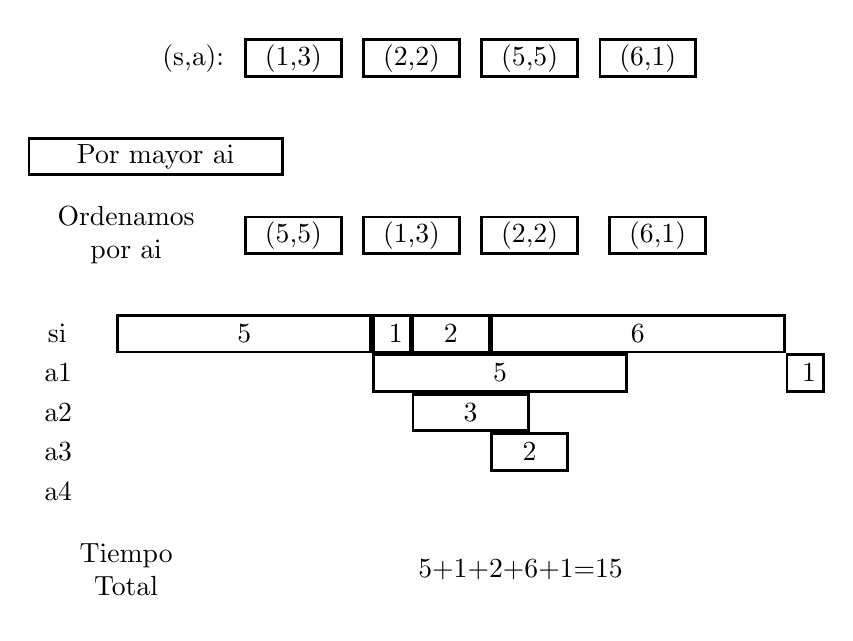
\begin{tikzpicture}
	% Paths, nodes and wires:
	\node[shape=rectangle, draw, line width=1pt, minimum width=1.215cm, minimum height=0.465cm] at (-0.625, 5.25){} node[anchor=center, align=center, text width=0.827cm, inner sep=6pt] at (-0.625, 5.25){(1,3)};
	\node[shape=rectangle, draw, line width=1pt, minimum width=1.215cm, minimum height=0.465cm] at (0.875, 5.25){} node[anchor=center, align=center, text width=0.827cm, inner sep=6pt] at (0.875, 5.25){(2,2)};
	\node[shape=rectangle, draw, line width=1pt, minimum width=1.215cm, minimum height=0.465cm] at (2.375, 5.25){} node[anchor=center, align=center, text width=0.827cm, inner sep=6pt] at (2.375, 5.25){(5,5)};
	\node[shape=rectangle, draw, line width=1pt, minimum width=1.215cm, minimum height=0.465cm] at (3.875, 5.25){} node[anchor=center, align=center, text width=0.827cm, inner sep=6pt] at (3.875, 5.25){(6,1)};
	\node[shape=rectangle, minimum width=0.965cm, minimum height=0.465cm] at (-2, 5.25){} node[anchor=center, align=center, text width=0.577cm, inner sep=6pt] at (-2, 5.25){(s,a):};
	\node[shape=rectangle, draw, line width=1pt, minimum width=3.215cm, minimum height=0.465cm] at (-2.375, 4){} node[anchor=center, align=center, text width=2.827cm, inner sep=6pt] at (-2.375, 4){Por mayor ai};
	\node[shape=rectangle, draw, line width=1pt, minimum width=3.215cm, minimum height=0.465cm] at (-1.25, 1.75){} node[anchor=center, align=center, text width=2.827cm, inner sep=6pt] at (-1.25, 1.75){5};
	\node[shape=rectangle, draw, line width=1pt, minimum width=1.215cm, minimum height=0.465cm] at (0.875, 3){} node[anchor=center, align=center, text width=0.827cm, inner sep=6pt] at (0.875, 3){(1,3)};
	\node[shape=rectangle, draw, line width=1pt, minimum width=1.215cm, minimum height=0.465cm] at (2.375, 3){} node[anchor=center, align=center, text width=0.827cm, inner sep=6pt] at (2.375, 3){(2,2)};
	\node[shape=rectangle, draw, line width=1pt, minimum width=1.215cm, minimum height=0.465cm] at (4, 3){} node[anchor=center, align=center, text width=0.827cm, inner sep=6pt] at (4, 3){(6,1)};
	\node[shape=rectangle, minimum width=2.465cm, minimum height=0.715cm] at (-2.75, 3){} node[anchor=center, align=center, text width=2.077cm, inner sep=6pt] at (-2.75, 3){Ordenamos por ai};
	\node[shape=rectangle, minimum width=0.715cm, minimum height=0.465cm] at (-3.625, 1.75){} node[anchor=center, align=center, text width=0.327cm, inner sep=6pt] at (-3.625, 1.75){si};
	\node[shape=rectangle, draw, line width=1pt, minimum width=0.465cm, minimum height=0.465cm] at (0.625, 1.75){} node[anchor=center, align=center, text width=0.077cm, inner sep=6pt] at (0.625, 1.75){1};
	\node[shape=rectangle, draw, line width=1pt, minimum width=0.965cm, minimum height=0.465cm] at (1.375, 1.75){} node[anchor=center, align=center, text width=0.577cm, inner sep=6pt] at (1.375, 1.75){2};
	\node[shape=rectangle, draw, line width=1pt, minimum width=1.215cm, minimum height=0.465cm] at (-0.625, 3){} node[anchor=center, align=center, text width=0.827cm, inner sep=6pt] at (-0.625, 3){(5,5)};
	\node[shape=rectangle, draw, line width=1pt, minimum width=3.715cm, minimum height=0.465cm] at (3.75, 1.75){} node[anchor=center, align=center, text width=3.327cm, inner sep=6pt] at (3.75, 1.75){6};
	\node[shape=rectangle, draw, line width=1pt, minimum width=3.215cm, minimum height=0.465cm] at (2, 1.25){} node[anchor=center, align=center, text width=2.827cm, inner sep=6pt] at (2, 1.25){5};
	\node[shape=rectangle, draw, line width=1pt, minimum width=1.465cm, minimum height=0.465cm] at (1.625, 0.75){} node[anchor=center, align=center, text width=1.077cm, inner sep=6pt] at (1.625, 0.75){3};
	\node[shape=rectangle, draw, line width=1pt, minimum width=0.965cm, minimum height=0.465cm] at (2.375, 0.25){} node[anchor=center, align=center, text width=0.577cm, inner sep=6pt] at (2.375, 0.25){2};
	\node[shape=rectangle, draw, line width=1pt, minimum width=0.465cm, minimum height=0.465cm] at (5.875, 1.25){} node[anchor=center, align=center, text width=0.077cm, inner sep=6pt] at (5.875, 1.25){1};
	\node[shape=rectangle, minimum width=0.715cm, minimum height=0.465cm] at (-3.625, 1.25){} node[anchor=center, align=center, text width=0.327cm, inner sep=6pt] at (-3.625, 1.25){a1};
	\node[shape=rectangle, minimum width=0.715cm, minimum height=0.465cm] at (-3.625, 0.75){} node[anchor=center, align=center, text width=0.327cm, inner sep=6pt] at (-3.625, 0.75){a2};
	\node[shape=rectangle, minimum width=0.715cm, minimum height=0.465cm] at (-3.625, 0.25){} node[anchor=center, align=center, text width=0.327cm, inner sep=6pt] at (-3.625, 0.25){a3};
	\node[shape=rectangle, minimum width=0.715cm, minimum height=0.465cm] at (-3.625, -0.25){} node[anchor=center, align=center, text width=0.327cm, inner sep=6pt] at (-3.625, -0.25){a4};
	\node[shape=rectangle, minimum width=2.465cm, minimum height=0.715cm] at (-2.75, -1.25){} node[anchor=center, align=center, text width=2.077cm, inner sep=6pt] at (-2.75, -1.25){Tiempo Total};
	\node[shape=rectangle, minimum width=2.465cm, minimum height=0.715cm] at (2, -1.25){} node[anchor=center, align=center, text width=2.077cm, inner sep=6pt] at (2, -1.25){5+1+2+6+1=15};
\end{tikzpicture}
\end{figure}